\section{Loi du chi carr� ($\chi^2$)}

\subsection{Loi du chi-2 � $n$ degr�s de libert�}
\begin{defi}
Soit $n$ variables al�atoires normales centr�es-r�duites $Z_i$, ind�pendantes les unes des autres et identiquement distribu�es: $Z_i  \mbox{ i.i.d.} \sim\norm(0,1)$, $i=1,2,\ldots,n$. Alors la variable form�e de la somme des carr�s de ces variables
$$Q_n = \sum_{i=1}^{n} Z_i^2 \sim \chi^2$$
suit une \emph{loi du $\chi^2$ � $n$ degr�s de libert�}.
\end{defi}

On note parfois $\chi^2(n)$ ou $\chi^2_n$ pour indiquer une loi du $\chi^2$ � $n$ degr�s de libert�

\begin{pro} La loi du $\chi^2$ � $n$ degr�s de libert� poss�de les propri�t�s suivantes
\begin{itemize}
	\item Son esp�rance vaut $n$
	%$\E (Q_n) = \sum_i\var (Z_i) = n$
	\item Sa variance vaut $2n$
	%$\var (Q_n)= \sum_i\var (Z_i^2) = 2n$
\end{itemize}
\end{pro}

%\begin{proof}
%$\chi^2=\frac{(n-1)s^2}{\sigma^2}=\frac{(n-1)\frac{\sum(x-\bar{x})^2}{n-1}}{\sigma^2}
%=\frac{\sum(x-\bar{x})^2}{\sigma^2} = \sum(\frac{x-\bar{x}}{\sigma})^2$
%\end{proof}
 
$$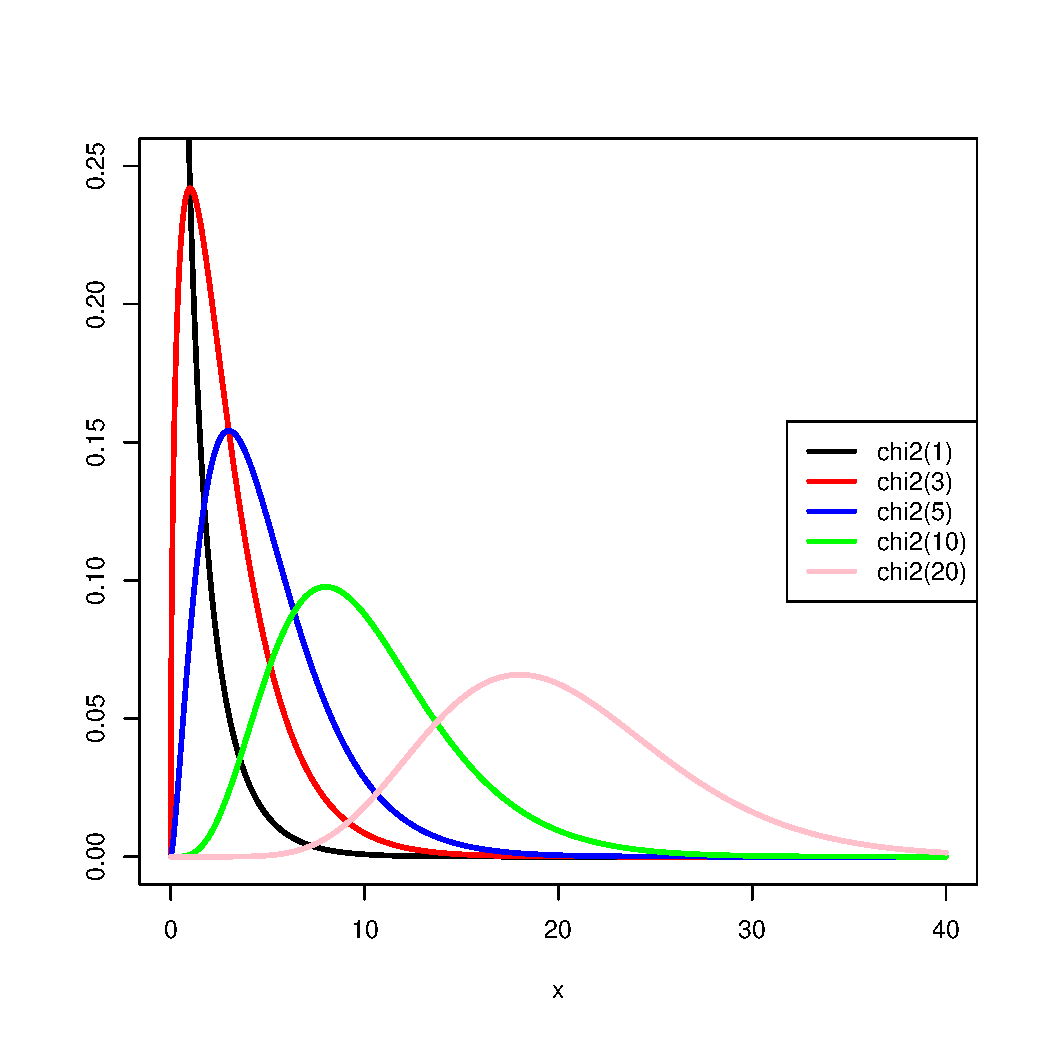
\includegraphics[scale=0.7]{chisquare}$$

\begin{rem}
La loi du chi-2 �tant d�finie comme une somme de carr�s, elle ne prend que des valeurs positives.
\end{rem}

Nous utiliserons la propri�t� suivante lorsque nous calculerons (cf. \ref{section:variance-estimation}
) un intervalle de confiance pour la variance d'une population.

\begin{pro}\label{pro:chi2}
La statistique $\chi^2$ � $n-1$ degr�s de libert� vaut
$$\chi^2 = \frac{(n-1)s^2}{\sigma^2}$$
o�\\
\begin{tabular}{ccl}
$\chi^2$ & = & variable chi-2 standard\\
$s^2$ &= &  variance de l'�chantillon\\
$\sigma^2$ & = & variance de la population\\
$n$ &= &  taille de l'�chantillon
\end{tabular}
\end{pro}


\subsection{Table du $\chi^2$}
\centerline{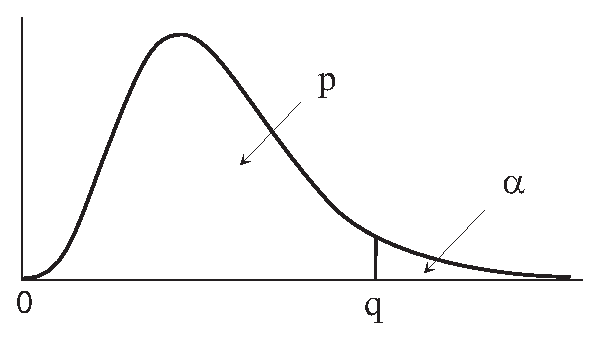
\includegraphics[width=10cm]{chi2b}}

Pour une variable $Q_n$ suivant une loi du $\chi^2$ � $n$ degr�s de libert�, $p = P(Q_n\leq q_{\alpha,n})$ et $\alpha = P(Q_n>q_{\alpha,n})$.
La relation entre $p$ et $\alpha$ est donn�e par 
$$p=1-\alpha$$

La table du $\chi^2$ en annexe \ref{sec:tablechideux} donne le seuil $q$ associ� � une erreur de premi�re esp�ce $\alpha$ (colonne) et un nombre de degr�s de libert� $n$ (ligne).

\begin{ex}
$P(Q_7 \leq q_{\alpha,7}) = 0.95$\\
Alors $\alpha=1-0.95=0.05$\\
Et donc $\quad q_{0.05,7} = 14.0671$
\end{ex}
